% ============================================
% SECTION 4: Conclusion
% ============================================
\section{Conclusão}

\begin{frame}{Conclusões}
\begin{center}
\Large
\begin{enumerate}
    \item \textbf{LA-CDIP Dataset}
    
    \vspace{0.25cm}
    Categorizado por layout visual para Zero-Shot Learning
    
    \vspace{0.5cm}
    
    \item \textbf{Metodologia com VDM}
    
    \vspace{0.25cm}
    Enforçando comparação de documentos como forma de classificação
    
    \vspace{0.5cm}

    \item \textbf{Benchmarking Sistemático}
    
    \vspace{0.25cm}
    Comparação entre modelos visuais e LLMs
    
\end{enumerate}
\end{center}
\end{frame}

\begin{frame}{Trabalhos Futuros}

\textbf{Trabalhos Futuros:}
\begin{itemize}
    \item Aumentar número de amostras
    \item Aumentar número de classes
    \item Incluir fontes adicionais de documentos
    \item PIBIC
\end{itemize}
\end{frame}

\begin{frame}{Publicações}
\begin{center}
\begin{tabular}{cc}
\tikz\node[draw=black, line width=.5pt, inner sep=0pt, drop shadow={opacity=0.1}]{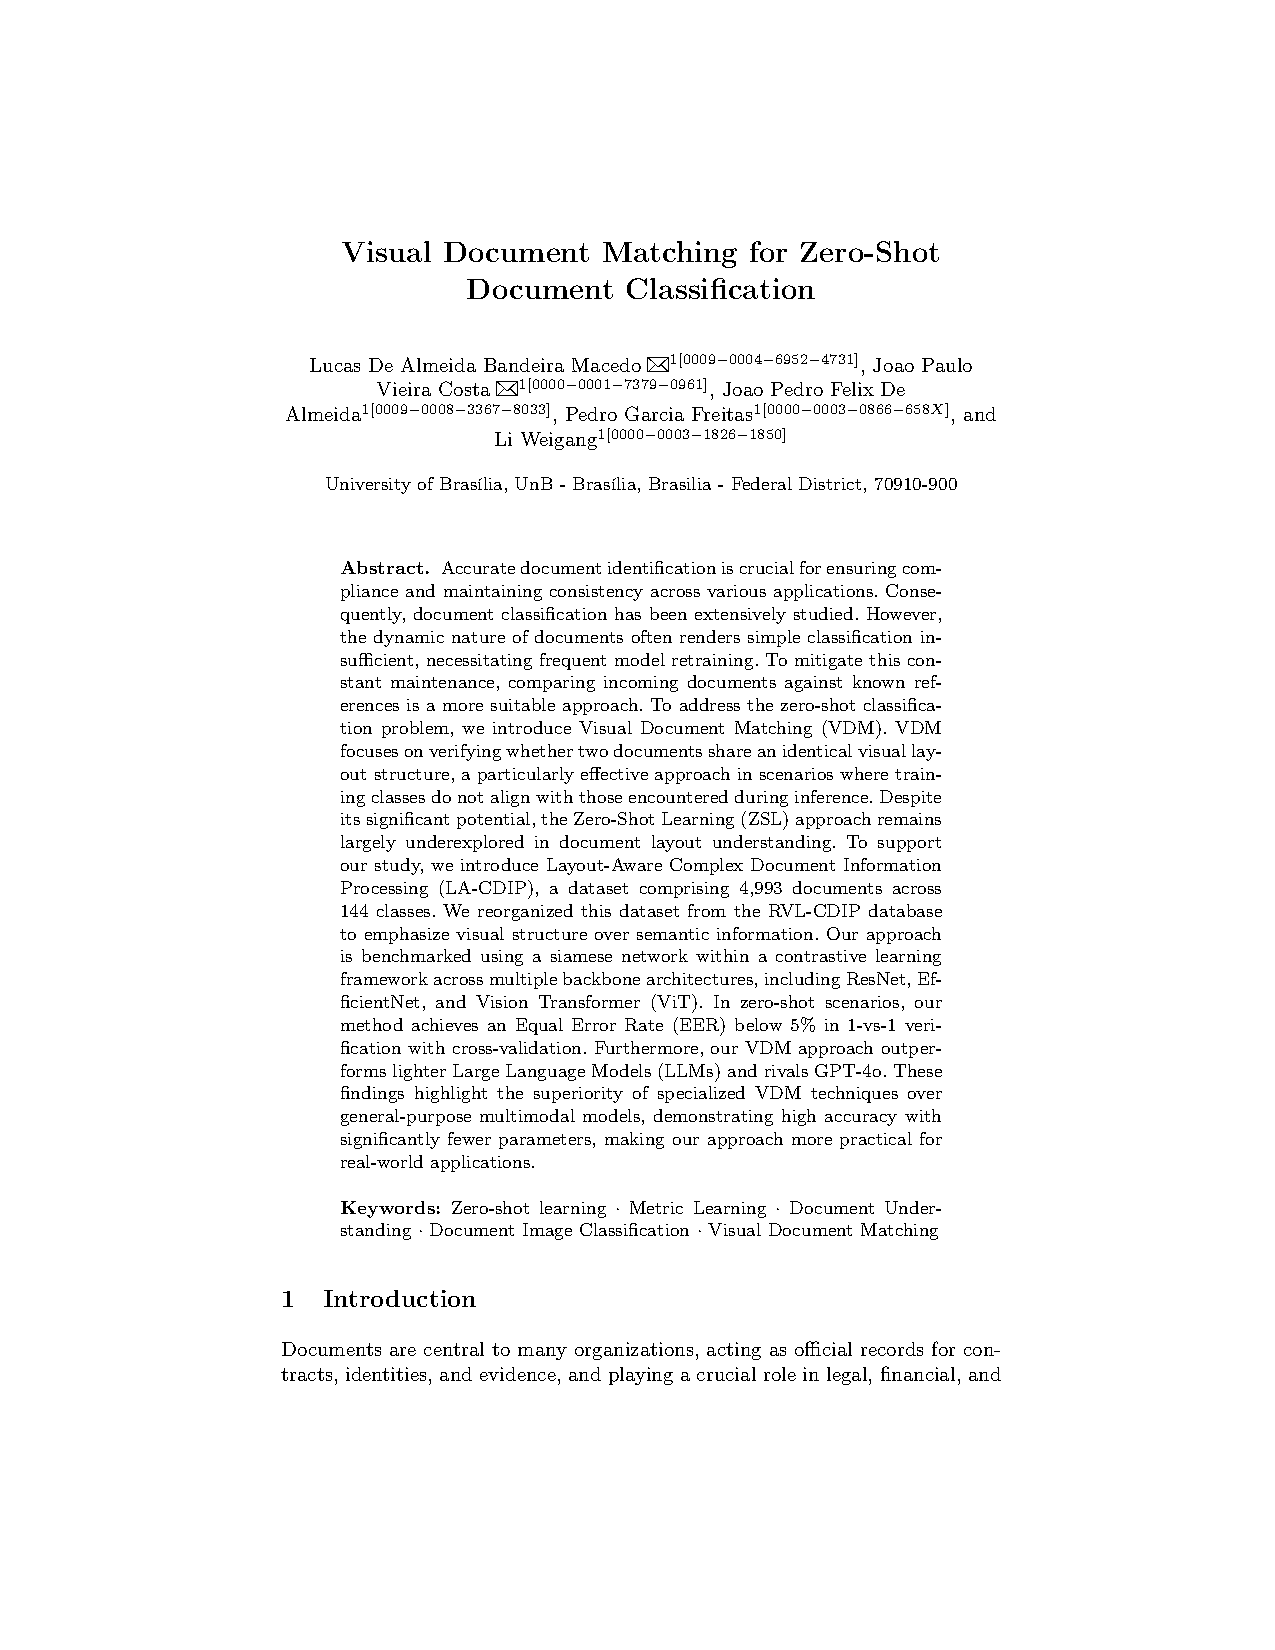
\includegraphics[height=0.7\textheight]{images-apresentacao/icdarwml-1pg.pdf}}; &
\tikz\node[draw=black, line width=.5pt, inner sep=0pt, drop shadow={opacity=0.1}]{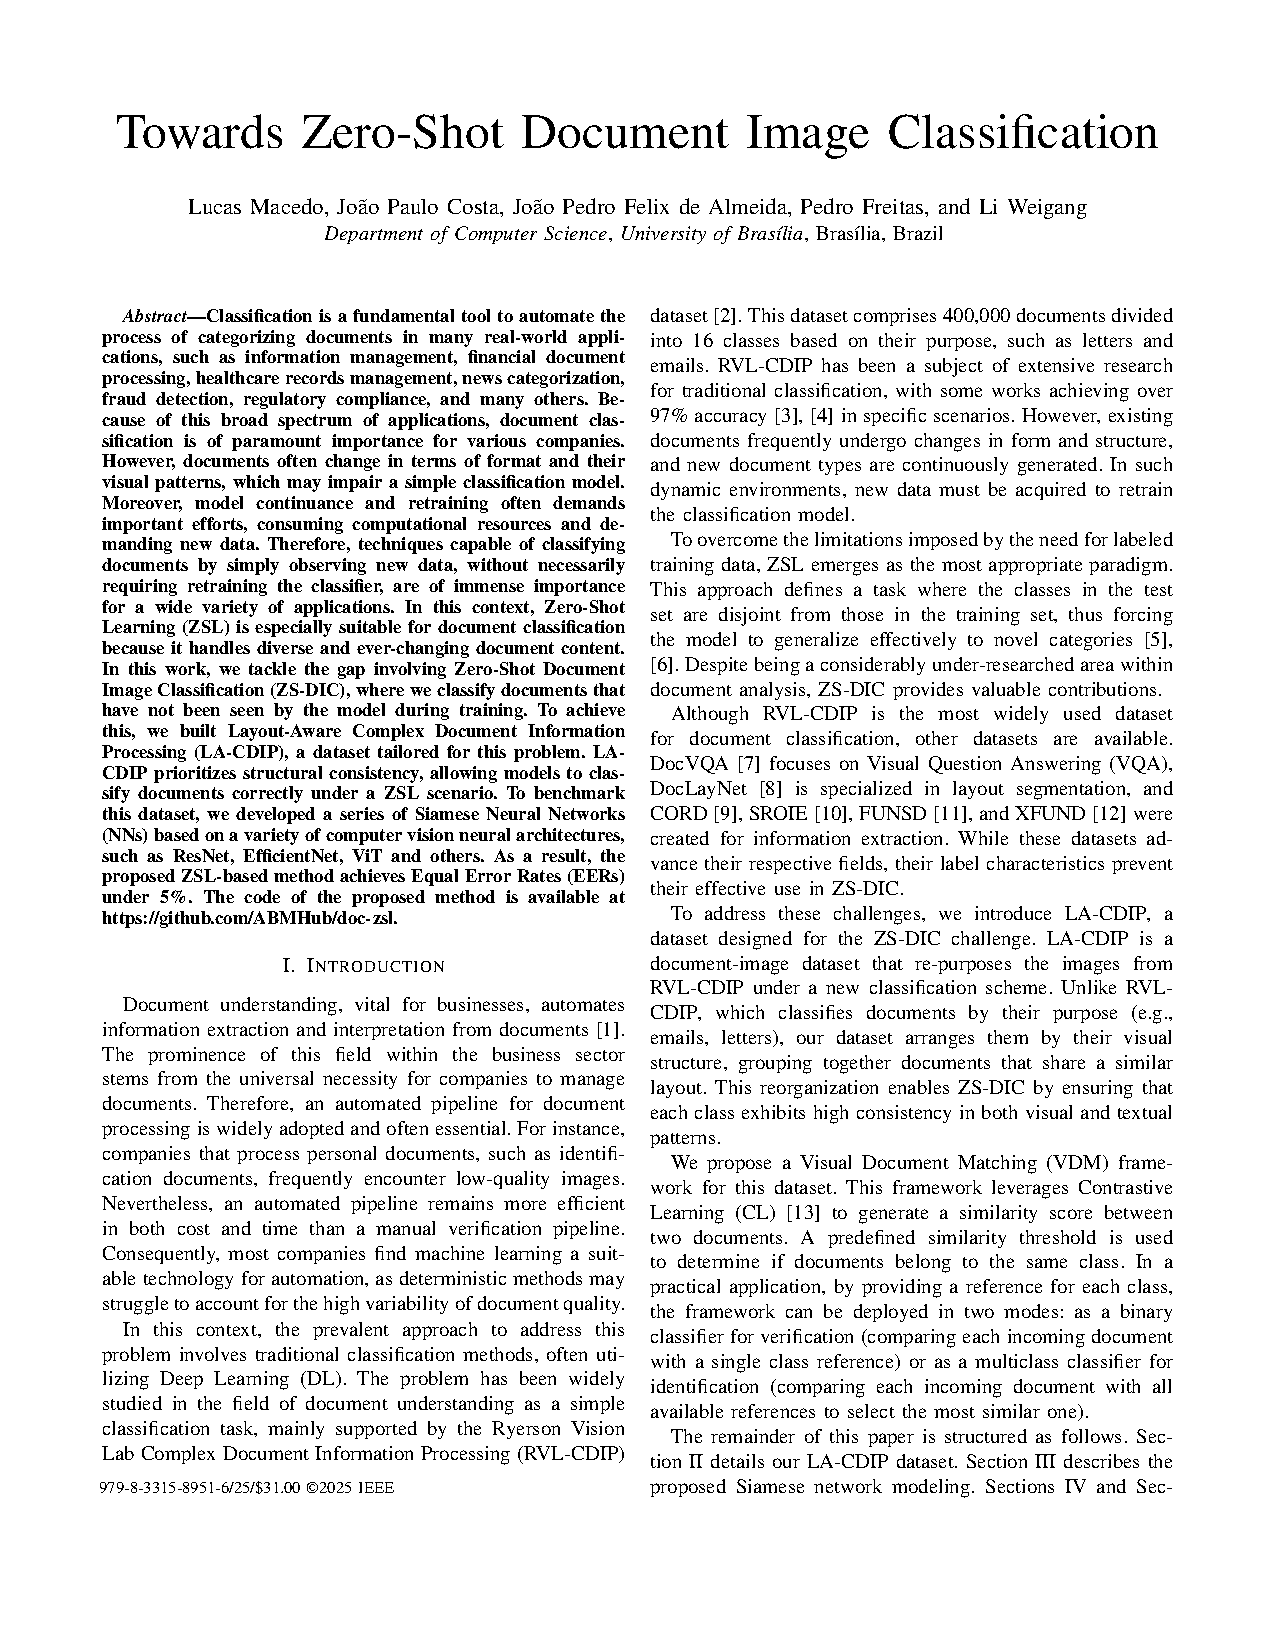
\includegraphics[height=0.7\textheight]{images-apresentacao/sibgrapi-1pg.pdf}}; \\
\textbf{ICDAR} & \textbf{SIBGRAPI}
\end{tabular}
\end{center}
\end{frame}

\begin{frame}{Publicações}
\begin{center}
\begin{tabular}{cc}
\tikz\node[draw=black, line width=.5pt, inner sep=0pt, drop shadow={opacity=0.1}]{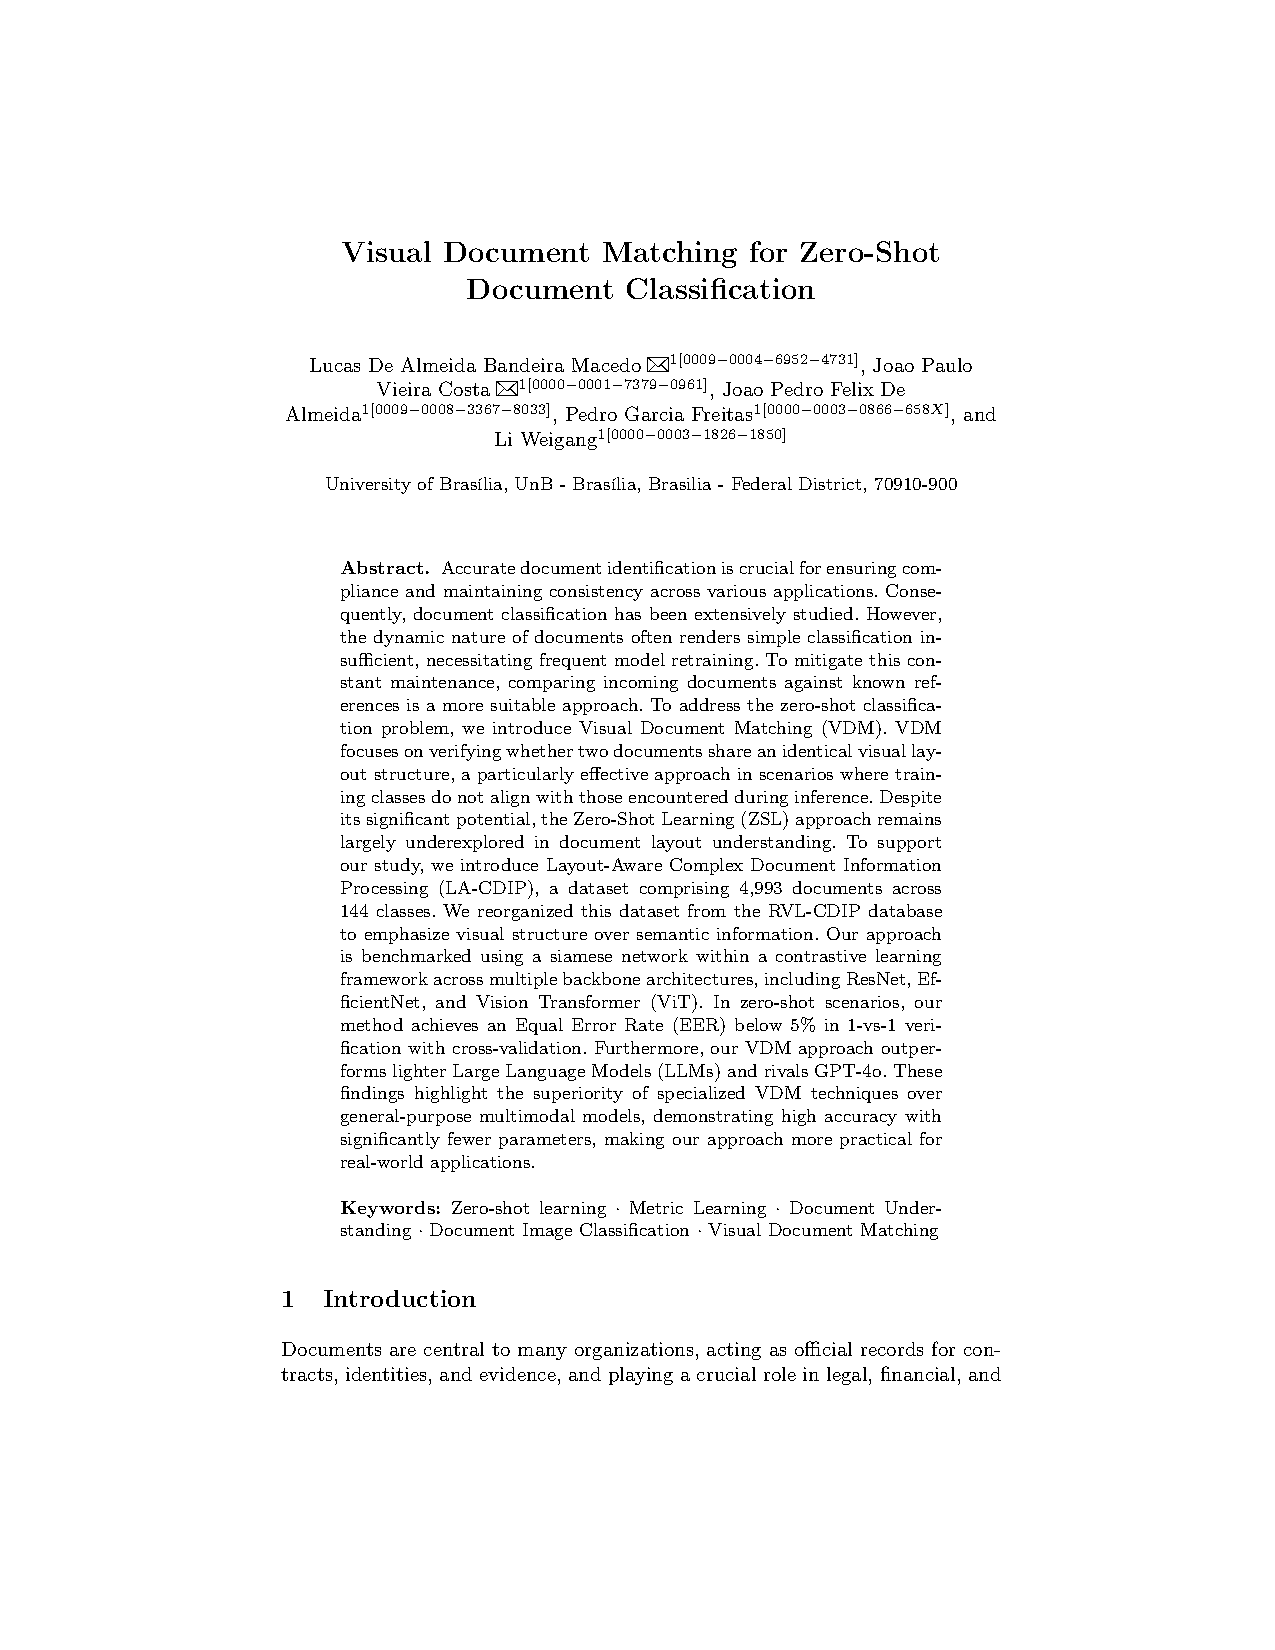
\includegraphics[height=0.7\textheight]{images-apresentacao/icdarwml-1pg.pdf}}; &
\tikz\node[draw=black, line width=.5pt, inner sep=0pt, drop shadow={opacity=0.1}]{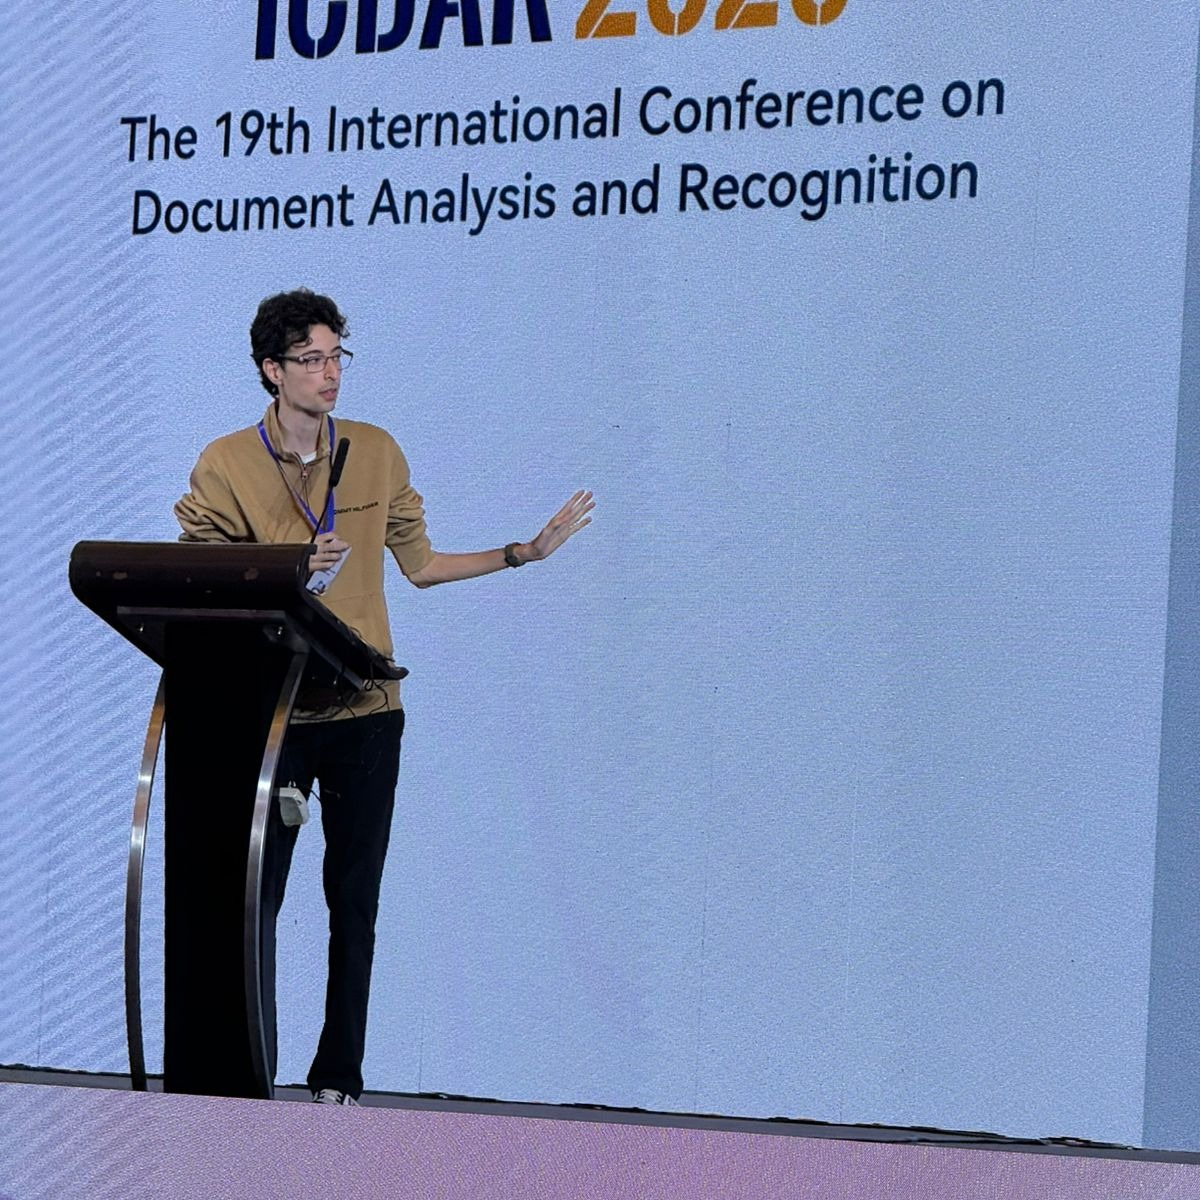
\includegraphics[height=0.7\textheight, trim={0 0 250 0}, clip]{images-apresentacao/foto-icdar.jpg}}; \\
\textbf{ICDAR} & \textbf{Apresentação}
\end{tabular}
\end{center}
\end{frame}
